\documentclass[11pt]{article}
\usepackage[T1]{fontenc}
\usepackage[a4paper,margin=1in]{geometry}
\usepackage{enumitem}
\usepackage{array}
\usepackage{hyperref}
\usepackage{amsfonts}
\usepackage{amsmath,amssymb}
\usepackage{tikz}
\usetikzlibrary{arrows.meta,positioning,fit,shapes,calc}
\usepackage[style=numeric,backend=biber]{biblatex}
\addbibresource{references.bib}

% Macros for real number symbols
\newcommand{\RD}{\mathbb{R}_{\mathrm{D}}}
\newcommand{\RC}{\mathbb{R}_{\mathrm{C}}}
\newcommand{\RFC}{\mathbb{R}_{\mathrm{FC}}}
\newcommand{\RI}{\mathbb{R}_{\mathrm{I}}}
\newcommand{\RH}{\mathbb{R}_{\mathrm{H}}}
\newcommand{\Rinit}{\mathbb{R}_{\mathrm{init}}}
\newcommand{\RES}{\mathbb{R}_{\mathrm{ES}}}
\newcommand{\RCF}{\mathbb{R}_{\mathrm{CF}}}
\newcommand{\Rb}{\mathbb{R}_{b}}
\newcommand{\RSD}{\mathbb{R}_{\mathrm{SD}}}
\newcommand{\RL}{\mathbb{R}_{\mathrm{L}}}
\newcommand{\RU}{\mathbb{R}_{\mathrm{U}}}
\newcommand{\RM}{\mathbb{R}_{\mathrm{M}}}
\newcommand{\RID}{\mathbb{R}_{\mathrm{ID}}}
\newcommand{\Rterm}{\mathbb{R}_{\mathrm{term}}}
\newcommand{\RDedComp}{\mathbb{R}_{\mathrm{DedComp}}}
\newcommand{\RTarski}{\mathbb{R}_{\mathrm{Tarski}}}
\newcommand{\RCauComp}{\mathbb{R}_{\mathrm{CauComp}}}
\newcommand{\REu}{\mathbb{R}_{\mathrm{E}}}
\newcommand{\Rformal}{\mathbb{R}_{\mathrm{formal}}}

\title{Real Number Definitions, Equivalence Classes, and Embeddings (No Countable Choice)}
\author{}
\date{}

\begin{document}
\maketitle

This document lists the first twenty-three constructive definitions of real numbers, partitions them into equivalence classes, and records the canonical embeddings. Note that while many equivalences hold in standard constructive mathematics (assuming Countable Choice, \(\mathsf{AC}_\omega\)), in plain Cubical Agda without \(\mathsf{AC}_\omega\), the hierarchy is more fractured (e.g., Cauchy reals are not provably Dedekind reals). General surveys and formalization resources include \cite{RichmanSurvey,TroelstraVanDalen1988,AgdaWiki}.

\section*{1. Definitions (1--33)}
\begin{enumerate}[leftmargin=*]
  \item $\mathbb{R}_\mathrm{D}$: Dedekind reals (located cuts of $\mathbb{Q}$) \cite{Dedekind1872,Bishop1967,BishopBridges1985,BridgesRichman1987,LubarskyRathjen2007,TomasiDedekind,Zanardo2012,MathOverflowLocales,Stout1976,nLabRealNumbers,Hall2010,Devillanova2021}.
  \item $\mathbb{R}_\mathrm{C}$: Cauchy reals (modulated Cauchy sequences of rationals, quotiented) \cite{Bishop1967,BishopBridges1985,LubarskyENTCS2007,Murray2022,MathOverflowDedekindCauchy,MathOverflowCauchyModulus,nLabCauchyReals}.
  \item $\mathbb{R}_\mathrm{E}$: Eudoxus reals (almost-homomorphisms $\mathbb{Z} \to \mathbb{Z}$) \cite{Arthan2004,Schanuel1992,Street2003,PROMYS2023,Fokma2021,Keskin2025,MathOverflowBauerHanson}.
  \item $\mathbb{R}_\mathrm{FC}$ / $\mathbb{R}_\mathrm{I}$: fast Cauchy reals / interval reals (Cauchy sequences with explicit moduli or nested rational intervals) \cite{Chernov2021,AbrialCansell2021,Weihrauch2000,WikiNestedIntervals}.
  \item $\mathbb{R}_\mathrm{CF}$: continued fraction reals (streams of partial quotients) \cite{BrilliantCF,WikiContinuedFraction,ConstructiveCF}.
  \item $\mathbb{R}_{b}$: coinductive base-$b$ reals (digit streams, e.g., binary/decimal) \cite{WiesnetKopp2022}.
  \item $\mathbb{R}_\mathrm{SD}$: signed-digit reals (streams over $\{-1,0,1\}$) \cite{Ambridge2024,TypeTopology,WiesnetKopp2022,Berger2011,Niqui2008,Kaganovsky1998,KoeppSchwichtenberg2022,BoehmEtAl1986,LubarskyRichman2015,BooijLocators,SchwichtenbergWiesnet2021,BergerSeisenberger2012,BergerLloyd2009,EscardoSimpson2014,WikiSignedDigit}.
  \item $\mathbb{R}_\mathrm{ID}$: interval domain reals (maximal elements of the interval domain) \cite{vanDerWeideFrumin2024,PattinsonMohammadian2021,deJong2023,BauerIntervalDomain,BauerTaylor2009,EdalatHeckmann1998,EdalatRealComputability,DiGianantonioReals,TaylorASDReals,Escardo1996,BauerKavkler2009}.
  \item $\mathbb{R}_\mathrm{L}$: lower reals (rounded lower sets of $\mathbb{Q}$) \cite{nLabOneSided,BlechschmidtHutzler2019,CoqConstructiveReals}.
  \item $\mathbb{R}_\mathrm{U}$: upper reals (rounded upper sets of $\mathbb{Q}$) \cite{nLabOneSided,BlechschmidtHutzler2019,CoqConstructiveReals}.
  \item $\mathbb{R}_\mathrm{M}$: MacNeille reals (double-negation closed cuts) \cite{MacNeille1937,nLabMacNeille,FourmanGrayson1982,Shulman2022}.
  \item $\mathbb{R}_\mathrm{H}$: HIT/HoTT-book reals (higher inductive type with universal property) \cite{HoTT2013,nLabHoTTReal,Booij2017,Booij2020,BauerHoTTReals2016,PrataliThesis}.
  \item $\mathbb{R}_\mathrm{ES}$: Escard\'o--Simpson reals (least Cauchy-complete subobject of $\mathbb{R}_\mathrm{D}$ containing $\mathbb{Q}$) \cite{EscardoSimpson2001,Booij2020}.
  \item $\mathbb{R}_\mathrm{formal}$: formal/locale reals (points of the locale of reals) \cite{MacLaneMoerdijk1992,Johnstone1982,Johnstone2002,PicadoPultr2012,Grossack2024,nLabRealNumbers}.
  \item $\mathbb{R}_\mathrm{init}$: initial sequentially modulated Cauchy-complete Archimedean ordered field \cite{EscardoSimpson2001,Booij2020,nLabArchimedean}.
  \item $\mathbb{R}_\mathrm{term}$: terminal Archimedean ordered field \cite{EscardoSimpson2001,MacLaneMoerdijk1992,nLabArchimedean}. Items 34 and 35 are distinct definitions with different construction proofs, but they result in the same object if the category is well-behaved.
  \item $\mathbb{R}_\mathrm{DedComp}$: Dedekind-complete ordered field (axiomatic characterization) \cite{MacLaneMoerdijk1992,Johnstone2002,BauerCompleteOrderedFields}.
  \item $\mathbb{R}_\mathrm{CauComp}$: Cauchy-complete ordered field (axiomatic characterization of the Cauchy completion) \cite{BishopBridges1985,TroelstraVanDalen1988}.
  \item $\mathbb{R}_\mathrm{Tarski}$: Archimedean Tarski group reals (characterization via Tarski's axioms) \cite{Tarski1951,Devillanova2021}.
  \item $[0,1]_\mathrm{coalg}$: unit interval as a terminal coalgebra \cite{EscardoSimpson2001,AdamekMiliusMoss2025,nLabCoalgebraInterval,Dusko2002}.
  \item $\mathbb{R}^+_\mathrm{coalg}$: positive reals as a terminal coalgebra \cite{EscardoSimpson2001,AdamekMiliusMoss2025,nLabCoalgebraInterval}.
  \item Sheaf-theoretic reals: the internal real numbers object in a topos \cite{MacLaneMoerdijk1992,Johnstone2002,Stout1976,Grossack2024,nLabRealNumbers}.
  \item Real numbers object (RNO) in a topos \cite{MacLaneMoerdijk1992,Johnstone2002,Stout1976,Grossack2024,nLabRealNumbers}. Items 41 and 42 are essentially the same mathematical object described from two different points of view (internal language vs.\ category theory).
  \item $\mathbb{R}_\mathrm{SDG}$: Smooth Reals (synthetic differential geometry). In Synthetic Differential Geometry, the reals are defined to include ``nilpotent'' infinitesimals (elements \(d\) where \(d^2 = 0\) but \(d \neq 0\)). These are distinct from standard Dedekind/Cauchy reals because they violate the field axiom \(x \neq 0 \implies x\) is invertible (nilpotents are not invertible). They are a distinct mathematical object internal to a smooth topos, not isomorphic to the usual Cauchy/Dedekind reals \cite{Kock2006,KosteckiSDG,MathOverflowSDG,nLabSmoothTopos}.
  \item $^*\mathbb{R}$: Hyperreals (non-standard analysis). These include infinite and infinitesimal numbers. While usually constructed classically (using ultrafilters), there are constructive approaches (e.g., Palmgren's constructive non-standard analysis) that result in a structure distinct from \(\mathbb{R}_\mathrm{D}\) or \(\mathbb{R}_\mathrm{C}\). They are strict extensions of the ordinary reals \cite{Robinson1966,Keisler1976,PalmgrenCNSA}.
  \item Predicative Reals: In systems stricter than Agda (like those prohibiting impredicativity), Dedekind cuts must be restricted (e.g., to ``generalized'' or ``weak'' cuts) to avoid circular definitions. The document hints at this with lower/upper reals (items 9, 10), but specific predicative formalizations often stand alone \cite{FefermanPredicative,BridgesMaietti2006,PaulinMohring1993}.
  \item $\mathbf{No}$: Surreal Numbers (Conway's construction). While the Surreals contain the Reals, the ``Real subset'' of the Surreals is a valid constructive definition of the reals. Inside \(\mathbf{No}\) there is a canonical embedded copy of \(\mathbb{R}\); this embedding can be used as yet another definition of the real line \cite{Conway1976,Gonshor1986,Mamane2004,Knuth1974,WikiSurreal}.
  \item Geometric Reals: Defined synthetically in Euclidean Geometry (e.g., Tarski's axioms for geometry, or Hilbert's axioms). Defined as ``points on a line'' rather than arithmetically. Constructively, relating ``points on a line'' to ``Dedekind cuts'' is a non-trivial project (requires the Cantor-Dedekind axiom) \cite{Tarski1951,Tarski1959,Beeson2015,Perout2013,WikiCantorDedekind}.
  \item Computable Reals (Turing): Specifically defined as ``Turing machines that output digits''. This is distinct from \(\mathbb{R}_\mathrm{C}\) because \(\mathbb{R}_\mathrm{C}\) allows \emph{any} function, whereas Computable Reals restrict the functions to computable ones. In strongly normalizing type theories, every \emph{definable} function is computable (meta-theoretically), so formalising computable reals inside such a system is natural. But this does not by itself make \(\mathbb{R}_\mathrm{C}\) ``the same'' as the usual Cauchy reals object; you still have to choose a semantic setting (e.g. an effective topos) where every function in the space is interpreted computably \cite{Turing1937,Aberth1980,Weihrauch2000,Geuvers2000}.
  \item Decimal / Base-10 Cauchy Reals: Reals as equivalence classes of decimal expansions; classically standard, but constructively they are just another representation type akin to digit-based reals \cite{Tao2016,BartleSherbert2011,WikiRealConstruction}.
  \item Apartness / Located Reals (Bishop Style): Reals as located, rounded lower cuts (or Cauchy sequences with an apartness relation). Bishop's ``Constructive Analysis'' uses a specific flavor of Cauchy reals (regular sequences with a fixed modulus of convergence, usually \(1/n\)). While often isomorphic to standard Cauchy reals, in a strict intensional type theory, the specific choice of modulus makes the type definition distinct \cite{Bishop1967,BishopBridges1985,BridgesMaietti2006,ResearchGateBishopReals}.
  \item Filter-based Completions: Reals as equivalence classes of Cauchy filters (or regular Cauchy filters) on~\(\mathbb{Q}\); conceptually close to Dedekind/Cauchy but more topological \cite{FarahWeiss2015}.
  \item Locale-of-Reals Variants: Several flavours exist internally: lower reals, upper reals, rounded reals, etc. Some topos texts distinguish a few different ``real objects'' as default~\cite{Vickers1996,FourmanGrayson1982,Johnstone1982,nLabRealNumbers}.
\end{enumerate}

\section*{2. Equivalence Classes (Provable without Countable Choice)}
Each class below consists of definitions that are often equivalent in constructive mathematics with \(\mathsf{AC}_\omega\). In plain Cubical Agda, equivalences between classes (e.g., A and B) may fail.

\subsection*{A. Dedekind-Type Completions}
$\mathbb{R}_\mathrm{D}$, $\mathbb{R}_\mathrm{formal}$, Sheaf-theoretic reals, and the real numbers object in a topos all present the Dedekind completion of $\mathbb{Q}$ via localized/topos-theoretic perspectives \cite{MacLaneMoerdijk1992,Johnstone1982,Johnstone2002,nLabRealNumbers,Grossack2024}.

\subsection*{B. Cauchy/HIT-Type Completions}
$\mathbb{R}_\mathrm{C}$, $\mathbb{R}_\mathrm{FC}$, $\mathbb{R}_\mathrm{I}$, $\mathbb{R}_\mathrm{H}$, $\mathbb{R}_\mathrm{init}$, $\mathbb{R}_\mathrm{ES}$, and (axiomatically) $\mathbb{R}_\mathrm{CauComp}$ represent the Cauchy completion, differing only in presentation (explicit modulus, higher inductive, universal property, or internal closure of $\mathbb{Q}$ within $\mathbb{R}_\mathrm{D}$) \cite{HoTT2013,Booij2017,Booij2020,Murray2022,SchwichtenbergWiesnet2021}.

\subsection*{C. Representation (Digit/Continued Fraction) Pre-Reals}
\(\mathbb{R}_\mathrm{CF}\), \(\mathbb{R}_{b}\), \(\mathbb{R}_\mathrm{SD}\), Decimal/Base-10 reals give concrete digit- or fraction-based streams. These are not literally ``the reals'' until quotiented; they are ``presentations of \(\mathbb{R}\)''. Raw types are not fields because of non-unique encodings, but their quotients by the appropriate equivalence relation coincide with Class B~\cite{Weihrauch2000,WiesnetKopp2022,MathStackConstructiveReals,BergerHou2007,Berger2011,Niqui2008,Kaganovsky1998,KoeppSchwichtenberg2022,BoehmEtAl1986,LubarskyRichman2015,BooijLocators,SchwichtenbergWiesnet2021,BergerSeisenberger2012,BergerLloyd2009}.

\subsection*{D. Coalgebraic Subspaces}
$[0,1]_\mathrm{coalg}$ and $\mathbb{R}^+_\mathrm{coalg}$ describe the unit interval and positive reals as terminal coalgebras. Constructively they model subspaces of $\mathbb{R}_\mathrm{D}$ but do not deliver the entire field without additional principles \cite{EscardoSimpson2001,AdamekMiliusMoss2025,nLabCoalgebraInterval,Rutten2000,EscardoSimpson2014}.

\subsection*{E. Generalized Cuts}
\(\mathbb{R}_\mathrm{L}\), \(\mathbb{R}_\mathrm{U}\), and \(\mathbb{R}_\mathrm{M}\) relax locatedness/density requirements. They contain \(\mathbb{R}\) as a canonical subobject (or as maximal elements) but are bigger structures and not isomorphic to \(\mathbb{R}\) as an ordered field~\cite{Vickers1996,MacNeille1937,BlechschmidtHutzler2019,FourmanGrayson1982,Shulman2022}.

\subsection*{F. Domain-Theoretic}
$\mathbb{R}_\mathrm{ID}$ sits in domain/locale theory. Its equivalence to Dedekind reals is not provable in plain Cubical Agda, so it remains a separate class. Note that in frameworks like Abstract Stone Duality or general Topos Theory, these often collapse into Class A (Dedekind-type) via duality results, but internally to Agda without extra axioms, the distinction is maintained \cite{AbramskyJung1994,EdalatHeckmann1998,vanDerWeideFrumin2024,PattinsonMohammadian2021,BauerIntervalDomain,DiGianantonioReals,TaylorASDReals}.

\subsection*{G. Axiomatic/Universal Characterizations}
\(\mathbb{R}_\mathrm{term}\), \(\mathbb{R}_\mathrm{DedComp}\), and \(\mathbb{R}_\mathrm{Tarski}\) capture Dedekind-like structures via universal properties or axioms. These are abstract characterizations; one still needs to show they are realized by some concrete construction. They coincide with the usual reals only once classical principles (e.g., choice) are assumed~\cite{MacLaneMoerdijk1992,Johnstone2002,BauerCompleteOrderedFields}.

\subsection*{H. Isolated/Unresolved}
$\mathbb{R}_\mathrm{E}$ (Eudoxus reals) currently lacks a constructive proof of equivalence with either Dedekind or Cauchy completions. We therefore mark it as isolated \cite{Arthan2004,Schanuel1992,PROMYS2023,Fokma2021,Keskin2025}.

\section*{2b. Diagrams}

\subsection*{Legend}
\begin{itemize}[leftmargin=*]
  \item Solid arrows: provable embeddings in plain Cubical Agda (no countable choice, no LEM).
  \item Dashed arrows: relationships that typically require countable choice or classical principles.
  \item ``quotient'' labels: representations coincide with Cauchy reals after quotienting the appropriate equivalence.
\end{itemize}

\subsection*{Diagram: Plain Cubical Agda (no CC/LEM)}

\begin{center}
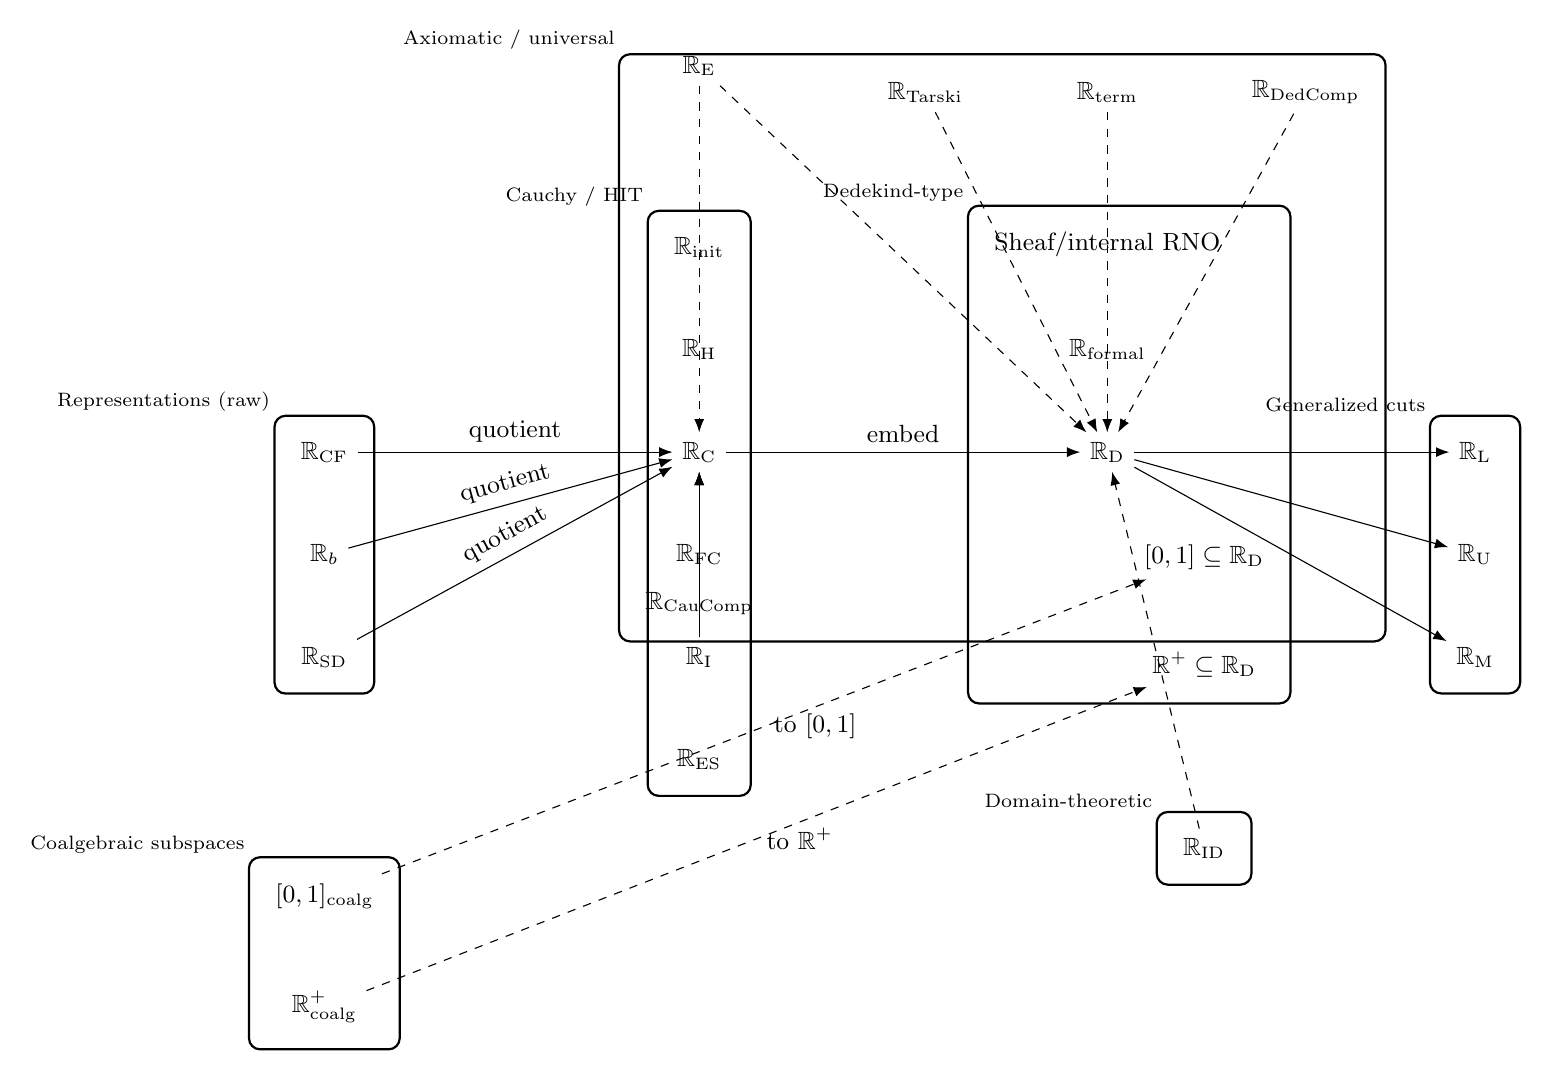
\begin{tikzpicture}[
  >=Latex,
  node distance=8mm and 12mm,
  every node/.style={font=\small},
  group/.style={draw, rounded corners, thick, inner sep=6pt},
  sublbl/.style={font=\scriptsize, inner sep=1pt},
  embed/.style={-Latex},
  cond/.style={-Latex, dashed},
]

% --- Nodes -----------------------------------------------------
% Cauchy / HIT (left-center)
\node (RC)   {\(\RC\)};
\node[below=of RC] (RFC) {\(\RFC\)};
\node[below=of RFC] (RI) {\(\RI\)};
\node[above=of RC] (RH) {\(\RH\)};
\node[above=of RH] (Rinit) {\(\Rinit\)};
\node[below=of RI] (RES) {\(\RES\)};

% Dedekind-type (center-right)
\node[right=45mm of RC] (RD) {\(\RD\)};
\node[above=of RD] (Rformal) {\(\Rformal\)};
\node[above=of Rformal] (RRNO) {Sheaf/internal RNO};
\node[below right=8mm and 0mm of RD] (Isub) {\([0,1] \subseteq \RD\)};
\node[below=of Isub] (RpSub) {\(\mathbb{R}^{+} \subseteq \RD\)};

% Representations (far left)
\node[left=40mm of RC] (RCF) {\(\RCF\)};
\node[below=of RCF] (Rb) {\(\Rb\)};
\node[below=of Rb] (RSD) {\(\RSD\)};

% Coalgebraic subspaces (bottom-left)
\node[below=25mm of RSD] (Icoalg) {\([0,1]_{\text{coalg}}\)};
\node[below=of Icoalg] (Rpcoalg) {\(\mathbb{R}^{+}_{\text{coalg}}\)};

% Generalized cuts (far right)
\node[right=40mm of RD] (RL) {\(\RL\)};
\node[below=of RL] (RU) {\(\RU\)};
\node[below=of RU] (RM) {\(\RM\)};

% Domain-theoretic (below center)
\node[below=18mm of RpSub] (RID) {\(\RID\)};

% Axiomatic / universal (top-center)
\node[above=14mm of RRNO] (Rterm) {\(\Rterm\)};
\node[right=12mm of Rterm] (RDedComp) {\(\RDedComp\)};
\node[left=12mm of Rterm] (RTarski) {\(\RTarski\)};
\node[below=14mm of RC] (RCauComp) {\(\RCauComp\)};

% Isolated / Eudoxus (top-left)
\node[above=18mm of Rinit] (REu) {\(\REu\)};

% --- Group boxes (fit) ----------------------------------------
\node[group, label={[sublbl]north west:Cauchy / HIT}] (GCB) [fit=(RC)(RFC)(RI)(RH)(Rinit)(RES)] {};
\node[group, label={[sublbl]north west:Dedekind-type}] (GDA) [fit=(RD)(Rformal)(RRNO)(Isub)(RpSub)] {};
\node[group, label={[sublbl]north west:Representations (raw)}] (GREP) [fit=(RCF)(Rb)(RSD)] {};
\node[group, label={[sublbl]north west:Coalgebraic subspaces}] (GCOA) [fit=(Icoalg)(Rpcoalg)] {};
\node[group, label={[sublbl]north west:Generalized cuts}] (GCUT) [fit=(RL)(RU)(RM)] {};
\node[group, label={[sublbl]north west:Domain-theoretic}] (GDOM) [fit=(RID)] {};
\node[group, label={[sublbl]north west:Axiomatic / universal}] (GAXI) [fit=(Rterm)(RDedComp)(RTarski)(RCauComp)] {};

% --- Proven embeddings (solid) --------------------------------
\draw[embed] (RC) -- node[above, sloped]{embed} (RD);
\draw[embed] (RFC) -- (RC);
\draw[embed] (RI) -- (RC);
\draw[embed] (RD) -- (RL);
\draw[embed] (RD) -- (RU);
\draw[embed] (RD) -- (RM);

% Representations quotient to Cauchy
\draw[embed] (RCF) -- node[above, sloped]{quotient} (RC);
\draw[embed] (Rb) -- node[above, sloped]{quotient} (RC);
\draw[embed] (RSD) -- node[above, sloped]{quotient} (RC);

% Coalgebraic to subspaces (caveats)
\draw[cond] (Icoalg) -- node[right]{to \([0,1]\)} (Isub);
\draw[cond] (Rpcoalg) -- node[right]{to \(\mathbb{R}^{+}\)} (RpSub);

% Axiomatic / domain / eudoxus --- conditional or unknown
\draw[cond] (Rterm) -- (RD);
\draw[cond] (RDedComp) -- (RD);
\draw[cond] (RTarski) -- (RD);
\draw[cond] (RCauComp) -- (RC);
\draw[cond] (RID) -- (RD);
\draw[cond] (REu) -- (RC);
\draw[cond] (REu) -- (RD);

\end{tikzpicture}
\end{center}

\subsection*{Diagram: With Countable Choice (illustrative collapse)}

\begin{center}
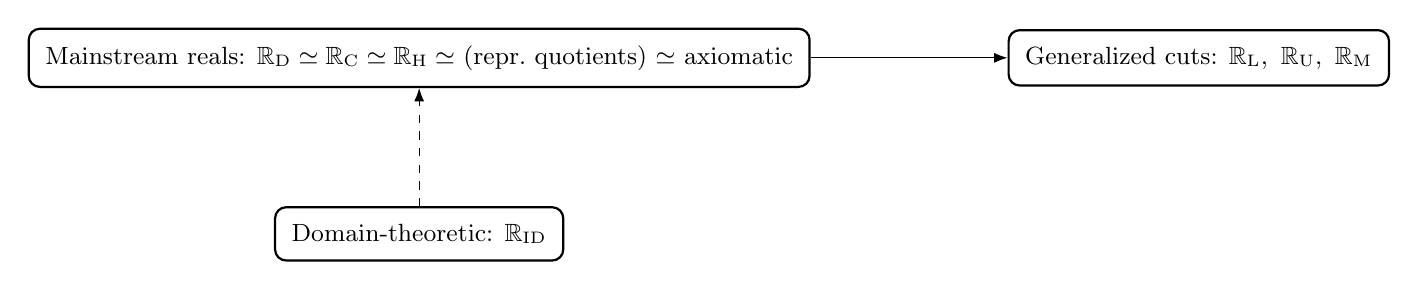
\begin{tikzpicture}[
  >=Latex,
  every node/.style={font=\small},
  group/.style={draw, rounded corners, thick, inner sep=6pt},
  cond/.style={-Latex, dashed}
]

\node[group] (Main) {Mainstream reals: $\RD \simeq \RC \simeq \RH \simeq$ (repr.\ quotients) $\simeq$ axiomatic};
\node[group, right=25mm of Main] (Cuts) {Generalized cuts: $\RL,\ \RU,\ \RM$};
\node[group, below=15mm of Main] (Dom) {Domain-theoretic: $\RID$};

\draw[-Latex] (Main) -- (Cuts);
\draw[cond] (Dom) -- (Main);

\end{tikzpicture}
\end{center}

\subsection*{ASCII Fallback}
\begin{verbatim}
Representations (raw) --quotient--> RC --embed--> RD --embed--> RL, RU, RM
     |                               \
     |                                \-- (subspaces) [0,1], R+ (via coalgebras; caveats)
     +-- R_CF, R_b, R_SD

Cauchy/HIT-type: RC, RFC, RI, [RH, R_init (distinct from RD constructively)], RES

Axiomatic: R_term, R_DedComp, R_Tarski, R_CauComp  ... (classically collapse to mainstream)

Domain-theoretic: R_ID  ... (related to RD; not provably equivalent)

Eudoxus: R_E  ... (isolated; classically related to Cauchy/Dedekind)
\end{verbatim}

\section*{2c. Corrections and Cautions}
\begin{itemize}[leftmargin=*]
  \item Embeddings go $\RD \to \RL,\ \RU$ by taking lower/upper cuts; the reverse is not constructive.
  \item Place $\RES$ with Cauchy-type (the Cauchy closure inside $\RD$), not with Dedekind-type.
  \item Keep $\RH$ and $\Rinit$ together and distinct from $\RD$ (they coincide only with extra principles).
  \item Treat $\RID$ as domain-theoretic and distinct in plain Cubical Agda; do not assert equivalence to $\RD$ without additional structure.
  \item Signed-digit/base-$b$/continued-fraction representations coincide with Cauchy only after quotienting and with suitable moduli.
\end{itemize}

\section*{3. Canonical Embeddings (No Countable Choice)}
\begin{itemize}[leftmargin=*]
  \item Cauchy into Dedekind: there is a canonical field embedding $\mathbb{R}_\mathrm{C} \hookrightarrow \mathbb{R}_\mathrm{D}$ that sends each Cauchy real to the located cut defined by its values \cite{BishopBridges1985,LubarskyENTCS2007,Lubarsky2007,MathOverflowDedekindCauchy}.
  \item Cauchy/HIT equivalences: $\mathbb{R}_\mathrm{FC}$, $\mathbb{R}_\mathrm{I}$, $\mathbb{R}_\mathrm{H}$, $\mathbb{R}_\mathrm{init}$, $\mathbb{R}_\mathrm{ES}$, and $\mathbb{R}_\mathrm{CauComp}$ are inter-definable and embed into $\mathbb{R}_\mathrm{C}$ (hence into $\mathbb{R}_\mathrm{D}$) \cite{HoTT2013,Booij2017,Booij2020,EscardoSimpson2001}.
  \item Representation quotients: the quotient of $\mathbb{R}_\mathrm{CF}$, $\mathbb{R}_{b}$, or $\mathbb{R}_\mathrm{SD}$ by the digit-equivalence relation embeds into $\mathbb{R}_\mathrm{C}$. Without quotienting there is a surjection obstruction due to non-unique encodings (Booij~\cite{BooijLocators} shows locators provide a choice-free signed-digit conversion for Dedekind reals with extra structure) \cite{Weihrauch2000,BergerHou2007,MathStackConstructiveReals,WiesnetKopp2022,Berger2011,Niqui2008,Kaganovsky1998,KoeppSchwichtenberg2022,BoehmEtAl1986,LubarskyRichman2015,SchwichtenbergWiesnet2021,BergerSeisenberger2012,BergerLloyd2009}.
  \item Dedekind to generalized cuts: taking lower (resp. upper) shadows gives embeddings $\mathbb{R}_\mathrm{D} \to \mathbb{R}_\mathrm{L}$ and $\mathbb{R}_\mathrm{D} \to \mathbb{R}_\mathrm{U}$. Composing with double-negation closure embeds into $\mathbb{R}_\mathrm{M}$ \cite{Vickers1996,nLabOneSided,nLabMacNeille,MacNeille1937}.
  \item Coalgebraic subspaces: maps $[0,1]_\mathrm{coalg} \to [0,1] \subseteq \mathbb{R}_\mathrm{D}$ and $\mathbb{R}^+_\mathrm{coalg} \to \mathbb{R}^+ \subseteq \mathbb{R}_\mathrm{D}$ exist, but surjectivity constructs require additional principles \cite{EscardoSimpson2001,AdamekMiliusMoss2025,nLabCoalgebraInterval}.
  \item Axiomatic to Dedekind/Cauchy: the objects $\mathbb{R}_\mathrm{term}$, $\mathbb{R}_\mathrm{DedComp}$, and $\mathbb{R}_\mathrm{Tarski}$ admit maps into $\mathbb{R}_\mathrm{D}$ matching their universal properties, yet converses rely on classical axioms and are not derivable constructively \cite{MacLaneMoerdijk1992,Johnstone2002,BauerCompleteOrderedFields,Devillanova2021}.
  \item Domain to Dedekind: $\mathbb{R}_\mathrm{ID}$ maps to $\mathbb{R}_\mathrm{D}$ via evaluation at maximal elements, but equivalence is unproven constructively \cite{AbramskyJung1994,EdalatHeckmann1998,BauerIntervalDomain,EdalatRealComputability}.
  \item Eudoxus: natural maps from $\mathbb{R}_\mathrm{E}$ into either $\mathbb{R}_\mathrm{C}$ or $\mathbb{R}_\mathrm{D}$ require countable choice for surjectivity and therefore remain dashed (non-provable) in this setting \cite{Arthan2004,PROMYS2023,Fokma2021,Keskin2025,MathOverflowBauerHanson}.
\end{itemize}

\section*{4. Higher Coinductive Types (HCITs) for Signed-Digit Reals}

Following Altenkirch~\cite{Altenkirch2024HCIT}, we explore defining the signed-digit reals as a \emph{Higher Coinductive Type} (HCIT)---the coinductive dual of HITs/QIITs. An HCIT has constructors (operations) and path constructors (equations built into the type), with its universal property being \emph{terminality} rather than initiality.

\subsection*{4.1 Signature}

An HCIT for the signed-digit interval $\mathbb{I}$ is specified by:
\begin{itemize}[leftmargin=*]
  \item \textbf{Operations:} $\mathsf{cons} : \mathrm{Digit} \to \mathbb{I} \to \mathbb{I}$, \; $\mathsf{inc}, \mathsf{dec} : \mathbb{I} \to \mathbb{I}$
  \item \textbf{Inc/dec equations} (carry/borrow propagation):
  \begin{align*}
    \mathsf{inc}(\mathsf{cons}\;(-1)\;x) &\equiv \mathsf{cons}\;0\;(\mathsf{inc}\;x) \\
    \mathsf{inc}(\mathsf{cons}\;0\;x) &\equiv \mathsf{cons}\;(+1)\;(\mathsf{cons}\;0\;x) \\
    \mathsf{inc}(\mathsf{cons}\;(+1)\;x) &\equiv \mathsf{cons}\;(+1)\;(\mathsf{inc}\;x)
  \end{align*}
  (symmetric for $\mathsf{dec}$)
  \item \textbf{Generation:} $\forall y.\;\exists d\,x.\;y \equiv \mathsf{cons}\;d\;x$
  \item \textbf{Completeness:} $\mathsf{cons}\;0\;x \equiv \mathsf{inc}\;y \;\Rightarrow\; \mathsf{cons}\;(-1)\;x \equiv \mathsf{cons}\;0\;y$
  \item \textbf{Separation:} $\mathsf{cons}\;(-1)\;x \equiv \mathsf{cons}\;0\;y \;\Rightarrow\; \mathsf{cons}\;0\;x \equiv \mathsf{inc}\;y$
  \item \textbf{Set truncation:} $\mathsf{isSet}(\mathbb{I})$
\end{itemize}

The carry/borrow equations $\mathsf{cons}\;(+1)\;(\mathsf{cons}\;(-1)\;x) \equiv \mathsf{cons}\;0\;(\mathsf{inc}\;x)$ are derivable from completeness + separation.

\textbf{Note:} The ``no-confusion'' axiom $\mathsf{cons}\;(-1)\;x \equiv \mathsf{cons}\;(+1)\;y \to \bot$ from Altenkirch's first attempt (slide~10) is \emph{false} in the quotient model: $[-1 :: 1^\omega]$ and $[+1 :: (-1)^\omega]$ both represent~$0$.

\subsection*{4.2 Type-theoretic rules}

\paragraph{Formation.} Given an HCIT signature $\Sigma = (\mathrm{Ops}, \mathrm{Eqs})$:
\[
  \frac{\Sigma : \mathsf{HCIT\text{-}Sig}}{\mathsf{HCIT}(\Sigma) : \mathsf{Type}}
\]

\paragraph{Introduction.} Operations become point constructors; equations become path constructors:
\[
  \frac{d : \mathrm{Digit} \quad x : \mathsf{HCIT}(\Sigma)}{\mathsf{cons}\;d\;x : \mathsf{HCIT}(\Sigma)}
  \qquad
  \frac{}{\mathsf{carry} : \mathsf{cons}\;(+1)\;(\mathsf{cons}\;(-1)\;x) \equiv \mathsf{cons}\;0\;(\mathsf{inc}\;x)}
\]

\paragraph{Elimination (terminality).} For any $\Sigma$-algebra $A$, there is a unique morphism into $\mathsf{HCIT}(\Sigma)$:
\[
  \frac{A : \Sigma\text{-Alg}}{\mathsf{corec}_A : A.\mathrm{Carrier} \to \mathsf{HCIT}(\Sigma)}
\]

\paragraph{Computation ($\beta$).}
$\mathsf{corec}_A(\mathsf{cons}_A\;d\;x) \equiv \mathsf{cons}\;d\;(\mathsf{corec}_A\;x)$

\paragraph{Uniqueness ($\eta$).}
$f : \Sigma\text{-Hom}\;A\;\mathsf{HCIT}(\Sigma) \;\Rightarrow\; f = \mathsf{corec}_A$

\subsection*{4.3 Encoding in Cubical Agda}

Native HCITs are unavailable in Cubical Agda. The quotient-of-codata encoding $\mathbb{I}_\mathrm{sd} = \mathbb{3}^\mathbb{N} / {\approx_\mathrm{sd}}$ recovers the equations but the corecursion principle (terminality) requires lifting through the quotient, which needs $\mathsf{AC}_\omega$ (countable dependent choice). This matches the obstruction for $\mathsf{lim}_{\mathbb{I}_\mathrm{sd}}$ documented in the codebase.

\paragraph{Stable Agda naming surface.}
To avoid notation drift between paper text and mechanization, the reviewer-facing API is frozen in
\texttt{Reals.SignedDigit.PaperB.Entrypoint}: the canonical identifiers are
\texttt{inc⁻¹}, \texttt{inc⁰}, \texttt{inc⁺¹}, \texttt{dec⁺¹}, \texttt{dec⁰}, \texttt{dec⁻¹},
\texttt{carry-compl}, \texttt{borrow-compl}, \texttt{sep-L}, \texttt{sep-R}, and \texttt{gen}.

\subsection*{4.4 Comparison with existing approaches}

\begin{center}
\begin{tabular}{@{}llccc@{}}
  \textbf{Approach} & \textbf{Type theory} & \textbf{Equalities} & \textbf{Corecursion} & \textbf{$\mathsf{AC}_\omega$-free} \\
  \hline
  Quotient of codata & Cubical Agda & via quotient & blocked & No \\
  Native HCIT & Cubical + primitive & native & native & Yes \\
  Coconditions & dTT/Narya & via coconditions & via comatching & Yes \\
  Greatest HITs & Clocked Cubical & guarded rec + HITs & guarded rec & Yes \\
\end{tabular}
\end{center}

\noindent\textbf{References:}
Altenkirch~\cite{Altenkirch2024HCIT} (HCIT proposal);
Lorenzen--Shulman~\cite{LorenzenShulman2024} (coconditions);
Kristensen--M{\o}gelberg~\cite{KristensenMogelberg2021} (Greatest HITs);
Ahrens--Capriotti--Spadotti~\cite{AhrensCapriottiSpadotti2015} (M-types in HoTT);
Narya docs~\cite{NaryaHigherTypes};
Displayed Type Theory~\cite{DisplayedTypeTheory2023};
Bronsveld~\cite{Bronsveld2025}.

\printbibliography

\end{document}
